\section{Macromolecular X-ray crystallography}
The discovery of X-ray diffraction by crystals by Max van Laue \cite{Friedrich1913-vx,Laue1913-sn} marked the origins of modern crystallography. However, it was not until the work of William Lawrence Bragg and William Henry Bragg that X-ray scattering could be translated into atomic positions \cite{Bragg1913-cx,Bragg1929-xp,Bragg1912-ht}. Since then, X-ray crystallography and the determination of atomic positions in organic and inorganic molecules of has come a long way and shaped the path for many 21\textsuperscript{st} century discoveries. Amongst those ground-breaking discoveries are the earliest structural models of biological molecules including DNA \cite{Watson1953-qw}, vitamin B12 \cite{Hodgkin1956-mx}, and the first protein structures \cite{Blundell1971-mv,Blake1965-ng,Perutz1960-qz,Kendrew1958-on}. These structure elucidations hallmarked the dawn of a new era in biological and biomedical research. At the time of writing, 124,551 structural models were determined by X-ray diffraction studies \cite{Berman2000-ua}, and thus X-ray crystallography is a key method in biological research.

\subsection{X-ray scattering}
X-rays are high energy photons part of the electromagnetic spectrum with a wavelength 0.1-100\AA\ \cite{Rupp2010-nc}. X-rays can be described as packets of travelling electromagnetic waves, whose electric field vector interacts with the charged electrons of matter \cite{Rupp2010-nc}. Such interaction, typically termed scattering, results in the diffraction of the incoming wave, which X-ray crystallography relies on.

In its simplest form, scattering of X-ray radiation can be explained in the scenario of exposure to a single free electron. The resulting scattering can be classed as elastic (Thomson scattering) or inelastic (Crompton scattering) \cite{Rupp2010-nc}. The latter --- scattering that results in a loss of energy of the emitting photon due to energy transfer onto the electron --- does not contribute to discrete scattering, the type of scattering X-ray diffraction relies on. In comparison, Thomson scattering does not result in a loss of energy of the emitting photon. This has significant effects, the incoming photon emits with the same frequency causing the electron to oscillate identically further enhancing the signal.

If we expand the example to include all electrons in an atom and expose the atom to X-ray radiation, our theory needs to be slightly expanded. Given that one or more electrons in an atom are not free but orbit around the atom's nucleus in a stable and defined manner, the distribution of these electrons around the nucleus determines the scattering of the incoming X-ray photons. The distribution of scattered photon waves is thus an overall representation of the probability distributions of each electron in the atom and is refered to as electron density $\rho(\boldsymbol{r})$. In X-ray scattering, it suffices to approximate the shape of the electron density to a sphere. If we now consider the emitting wave $\boldsymbol{s_1}$ of an X-ray photon scattered by any position $\boldsymbol{r}$ in the electron density of an atom, then the phase difference $\Delta\varphi$ to the incoming wave $\boldsymbol{s_0}$ can be described by \cref{eq:phase_difference} \cite{Rupp2010-nc}.

\begin{equation}
    \Delta\varphi=2\pi\left(\boldsymbol{s_1}-\boldsymbol{s_0}\right)\boldsymbol{r}=2\pi \cdot \boldsymbol{S}\boldsymbol{r}
    \label{eq:phase_difference}
\end{equation}

If more than one electron in an atom's electron density scatter the incoming X-ray wave, then the emitting partial waves can be described by the atomic scattering function $f_s$ (\cref{eq:atomic_scattering_factor}), which describes the interference of all scattered waves \cite{Rupp2010-nc}. The total scattering power of an atom is proportional to the number of electrons and element-specific with heavier atoms scattering more strongly. Given the approximation of a centrosymmetric electron density, the atomic scattering function is also symmetric.

\begin{equation}
    f_s=\int\limits_{\boldsymbol{r}}^{V(atoms)}\rho\left(\boldsymbol{r}\right) \cdot e^{2\pi\\i\boldsymbol{S}\boldsymbol{r}} \cdot d\boldsymbol{r}
    \label{eq:atomic_scattering_factor}
\end{equation}

With an enhanced understanding of X-ray scattering of electrons orbiting a single atom, it is important to consider X-ray scattering of adjacent atoms, such as it is typically found in molecules. If the electromagnetic wave of a X-ray photon excites all electrons of adjacent atoms, then the resulting partial waves result in constructive or destructive interference. Maximal interference can be obtained when all partial waves are in phase, and maximal destructive interference when out-of-phase. This leads to varying intensities of the emitting X-ray photon at different points in space. To obtain the overall scattering power $F_s$ of all contributing atoms, \cref{eq:atomic_scattering_factor} needs to be modified to include the sum over all atoms $j$ as described in \cref{eq:total_scattering_power}.

\begin{equation}
    F_s=\sum_{j=1}^{atoms}f_{s,j}^0 \cdot e^{2\pi\\i\boldsymbol{S}\boldsymbol{r}_j}
    \label{eq:total_scattering_power}
\end{equation}

If we now translate our hypothetical experiment into a crystal lattice then our understanding described in \cref{eq:total_scattering_power} needs to be expanded from a 1-dimensional distance vector $\boldsymbol{r}$ to the three dimensional lattice translation vectors $\boldsymbol{a}$, $\boldsymbol{b}$ and $\boldsymbol{c}$. The Laue equations (\cref{eq:laue_equations}) do exactly that and ultimately determine the positions of the diffraction peaks in 3-dimensional space.

\begin{equation}
    \boldsymbol{S} \cdot \boldsymbol{a}=n_1, \quad \quad \boldsymbol{S} \cdot \boldsymbol{b}=n_2, \quad \quad \boldsymbol{S} \cdot \boldsymbol{c}=n_3
    \label{eq:laue_equations}
\end{equation}

\begin{equation}
    n\lambda=2d_{hkl}sin\theta
    \label{eq:bragg_equation}
\end{equation}

Such determination is possible through the findings made by \textcite{Bragg1913-cx}, who identified the relationship between the scattering vector $\boldsymbol{S}$ and the planes in the crystal lattice. Today, this relationship is defined by the Bragg equation (\cref{eq:bragg_equation}) \cite{Bragg1913-cx}, which allows us to interpret X-ray diffraction as reflections on discrete lattice planes, which relates the diffraction angle $\theta$ to the lattice spacing $d_{hkl}$ (\cref{fig:introduction_bragg}) \cite{Rupp2010-nc}. For maximum diffraction $n$ needs to be integer multiples to result in maximum constructive interference of wavelength $\lambda$.

\begin{figure}[H]
    \centering
    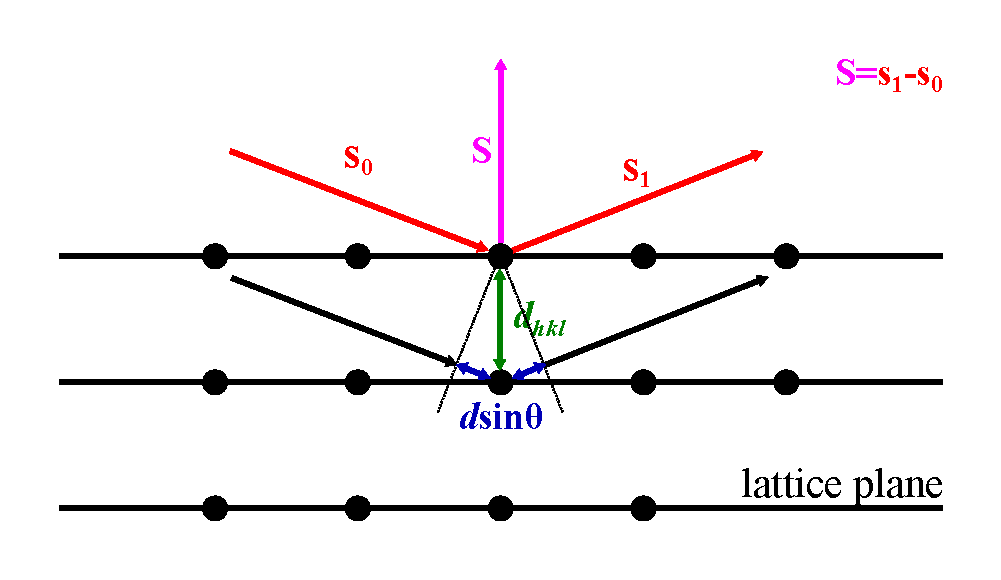
\includegraphics[width=0.7\textwidth]{introduction_bragg.pdf}
    \caption{Schematic of Bragg scattering.}
    \label{fig:introduction_bragg}
\end{figure}

Lastly, if the hypothetical model is expanded to molecular crystals, then the total scattering from the unit cell is merely a summation of all molecular unit cell scattering contributions in the crystal. Mathematically, this results in \cref{eq:total_scattering_power} being generalised to \cref{eq:structure_factors} through the application of the Laue equations (\cref{eq:laue_equations}) to express the scattering vector $\boldsymbol{S}\boldsymbol{r}_j$ as Miller indices of the reflection planes $\boldsymbol{h}\boldsymbol{x}_j$.

\begin{equation}
    F_h=\sum_{j=1}^{atoms}f_{s,j}^0 \cdot e^{2\pi\\i\boldsymbol{h}\boldsymbol{x}_j}
    \label{eq:structure_factors}
\end{equation}

The structure factor equation defines the scattering power from a crystal in a given reciprocal lattice direction $\boldsymbol{h}$. The scattering is enhanced by the number of repeating units of lattice translation vectors $\boldsymbol{a}$, $\boldsymbol{b}$ and $\boldsymbol{c}$, and thus the overall scattering power is proportional to the number of unit cells in the crystal.

It should be noted that \cref{eq:structure_factors} is a simplification of the problem at hand. In reality, instrument and experimental corrections need to be applied to the structure factor equation. A correction factor for each experiment-dependent parameter needs to be applied to the structure factor equation. However, in the scope of this work the details of such correction factors do not need to be discussed.

\begin{equation}
    \rho(x,y,z)=\frac{1}{V}\sum_{h=0}^{+\infty}\sum_{k=-\infty}^{+\infty}\sum_{l=-\infty}^{+\infty}\boldsymbol{F}(hkl)\cdot e^{-2\pi\\i(hx+ky+lz)}
    \label{eq:electron_density}
\end{equation}

Since complex structure factors describe the molecular structure in the reciprocal space domain, the conversion to the real space domain in form of electron density is required. This can be conveniently done through the bijective Fourier transform, which allows to convert complex structure factors to electron density and vice versa without the loss of any information \cite{Rupp2010-nc}. Thus, electron density can be obtained from the complex structure factors using \cref{eq:electron_density}. The normalisation factor $1/V$ provides the correct units for the electron density $\rho(x,y,z)$.

\subsection{From crystal to structure}
In X-ray crystallographic experiments, X-ray radiation is measured using light detectors. However, the measurement taken is incomplete. Light detectors only capture the intensity of the scattered X-ray photons but crucially lose the phase information. The latter is essential for atomic reconstruction of the molecule in the crystal, and thus needs to be obtained.  In \gls{mx}, experimentalists have a number of alternative techniques to compensate for the lost phase information. 

Prior to the big advances in computing power and the successful elucidation of many protein structures, \gls{mx} crystallographers primarily recovered the lost phase information through Direct Methods or Experimental Phasing \cite{Rupp2010-nc}. Today, the most popular method to recovering the lost phase information is \gls{mr} \cite{Rossmann2001-yw,Rossmann1990-am}. In a \Gls{mr} search, a known structure (`search model') similar to the unknown is relocated in the unit cell until the solution with the best fit between calculated and observed diffraction data is obtained \cite{Rupp2010-nc}. A 6-dimensional search, i.e. a simultaneous rotation and translation search, is possible \cite{Kissinger1999-ho,Glykos2000-gc,Read2001-nu}, however computationally very expensive and less suitable for challenging cases. In comparison, most modern crystalloraphic applications opt for two distinct sub-searches, the rotation search to orient the search model within the unit cell followed by the translation search to locate it \cite{Rupp2010-nc}. The benefits over a combined search include search-specific target functions that enable increased sensitivity and additional terms to compensate for imperfect data. 

The most successful \gls{mr} algorithms perform the rotation and translation searches using Patterson methods or Maximum Likelihood functions. Patterson methods --- originally developed by \textcite{Rossmann1962-ou} --- rely on the use of a map of vectors between the scattering atoms, which can be determined for the calculated and observed structure factor amplitudes. Patterson vectors can be sub-classed as intra- and inter-molecular vectors. A distinct separation of the observed vectors is impossible. However, inter-molecular vectors appear further away from the central peak of self-vector (vector from atom to itself) in the Patterson map \cite{Rupp2010-nc}. The calculated Patterson vectors for the search model allow for a clearer distinction between the intra- and inter-molecular vectors. If the search model is placed in a large unit cell, then inter-molecular vectors must scale with the unit cell dimension \cite{Rupp2010-nc}. Ultimately, using the intra-molecular Patterson vectors, the search probe can be oriented against the experimentally determined Patterson vectors. Similarly, the inter-molecular vectors can be used to identify the correct translation of the search probe. Patterson methods are very sensitive to small orientation errors of the search probe \cite{Rupp2010-nc}. Thus, orientations with the highest vector peak overlaps are trialed in the subsequence translation search.

In comparison to the Patterson methods, Maximum Likelihood methods do not rely on inter-atomic vectors in Patterson maps. Instead, Maximum Likelihood methods make use of Bayes' theorem \cite{Bayes1763-ox} to compare calculated structure factors and observed structure factor amplitudes directly \cite{Read2001-nu}. Bayes' theorem in crystallographic Maximum Likelihood methods is applied to compute the likelihood that an experimental value is observed given the current search model. The maximal likelihood indicates the best search model given the observed experimental data. Since the search model likelihood term is the product of many individual probabilities, which are difficult to represent computationally due to floating point representations, the log of the likelihood is commonly used \cite{Rupp2010-nc}. The major advantage of Maximum likelihood methods over Patterson methods centres on the more realist target functions, which consider errors and incompleteness of the search model, applies bulk solvent correction and conducts multi-model searches \cite{Read2001-nu}. The latter is of particularl relevance since the Maximum likelihood rotation function can thus consider already placed search model probes in a fixed position whilst trialling additional ones \cite{Storoni2004-ed}, which proves to be a major advantage over Patterson methods.  Furthermore, likelihood target functions consider the structural variance of multiple superposed models in an ensemble search model, which is used to weight structure factors at the various positions to improve the overall likelihood term \cite{Read2001-nu}. 

The initial electron density map after \gls{mr} is almost always inaccurate because of the search model-based phases. Inaccuracies arise from experimental errors, model incompleteness, low signal-to-noise or model bias. Thus, approaches for improving the phases used to calculated the initial electron density map have been developed and are routinely applied in \gls{mx}. Density modification describes a set of methods that improve the obtained electron density typically by applying statistical corrections to electron density distributions. These corrections are based on prior knowledge or assumptions of the physical properties of macromolecular structures \cite{Rupp2010-nc}. This process can transform initially poor or uninterpretable initial electron density maps to high quality ones. Three pre-dominant density modification approaches exist: solvent flattening, histogram matching and the ``sphere-of-influence'' method. Solvent flattening is an approach first proposed by \textcite{Wang1985-zu}, which exploits the fact that solvent regions in protein crystals are disordered, and thus differ in electron density volume from macromolecule-containing regions. If solvent electron density is set to a constant, then it is essentially flattened which will result in improved structure factors with improved phases and thus improved electron density. Histogram matching \cite{Lunin1988-lx} exploits the defined characteristics of an electron density distribution determined from sets of proteins at the same resolution, irrespectivce of individual structural details. The electron density distribution for noisy maps are Gaussian-shaped. In contrast, the electron density distribution of a feature-defined map is positively skewed. The ``sphere-of-influence'' method was introduced by \textcite{Sheldrick2002-tx} and classifies solvent and protein electron density by observing its variance across the shell surface of a 2.42\AA\ sphere (dominant 1-3 atom distance in macromolecular structures). If the sphere is positioned in the disordered solvent region typically found in intermolecular channels, the density variance will be low. Thus, this approach allows to smoothen solvent-containing regions of the electron density \cite{Sheldrick2002-tx}. Independent of the density modification strategy applied, it is important to understand that improvements to the electron density map anywhere lead to improvements everywhere by transferral of information from one part of the map to another \cite{Terwilliger2000-sz}.

A second approach to improving the initial electron density is termed Refinement. Iteratively, the placed search model is optimised to better describe the experimentally observed data. This optimisation problem is typically broken down into three main steps: the definition of the model parameters, the scoring function and the optimisation method. The model parameters describe the crystal and its content and can be subdivided into atomic and non-atomic model parameters \cite{Afonine2012-bg}. These parameters combined are used to score the current model. The scoring function relates the experimental data to the model parameters. The scoring function contains two primary terms, the refinement data target and an \textit{a priori} knowledge term. The former defines a target function that assesses the similarity between calculated and experimental structure factors. The target function is commonly a Maximum Likelihood-based function that considers missing or incomplete data \cite{Murshudov2011-ww,Afonine2012-bg}. The \textit{a priori} knowledge term in the scoring function defines the properties of a good model by including stereochemical property terms. Lastly, optimisation methods provide tools to vary the model parameters to better fit the experimental data. Different optimisation techniques can be used depending on the severity of model parameter alteration, which generally depend on the entrapment of states in local energy minima. The three steps combined form a macrocycle that iteratively modifies the model to optimise its fit to the experimental data. This ultimately improves both the electron density map interpretability and model quality. \gls{mx} refinement can be performed in structure-factor-based reciprocal space and electron-density-based real space \cite{Afonine2012-bg}. A combination allows global and local refinement strategies and enables grid-like searches to optimise the model parameters until convergence.

Once initial phase information is improved through refinement and density modification, attempts can be made to build atomic model coordinates into the electron density map. This process is typically coupled with refinement or density modification to iteratively improve the quality of the partially built model and the electron density map \cite{Rupp2010-nc}. A small number of distinct algorithms are currently used to automatically build atomic coordinates into electron density: main-chain autotracing \cite{Sheldrick2010-cx}, fitting pseudo-atoms into electron density \cite{Lamzin2001-cn}, or fitting reference coordinates with similar electron density maps \cite{Terwilliger2004-ig,Cowtan2006-xv}. In essence, all algorithms attempt to maximise the number of correctly identified and placed atomic coordinates into available electron density. Whilst autotracing solely builds main-chain peptides, the other two approaches rely on sequence information to also build side-chains. Independent of the complexity of the model building task, the higher the resolution and the more complete the initial starting model, the less ambiguous and challenging this overall task becomes \cite{Rupp2010-nc}. 

\subsection{Unconventional Molecular Replacement}
The process of macromolecular structure determination via conventional \gls{mr} has been outlined previously. Search models are typically derived from structural homologs identified by sequence similarity to the crystallised target \cite{Rupp2010-nc}. However, with decreasing sequence similarity between homologs, it becomes more challenging to identify structural templates suitable for \gls{mr}. Furthermore, experimental phasing approaches to circumvent the absence of \gls{mr} templates can be expensive, unsuccessful and very challenging for certain protein targets, and thus remain unfeasable to pursue at times. Under such circumstances, alternative approaches are required, which are referred to as ``unconventional'' \gls{mr} approaches from here onwards. The unconventional \gls{mr} approach most relevant to the work presented in this thesis utilises the 3-dimensional structure prediction of a protein target starting from its sequence \cite{Qian2007-vo,Rigden2008-vo,Das2009-uz}. 
 
\section{\textit{Ab initio} protein structure prediction}
The folding of protein structures is commonly described by the folding funnel hypothesis \cite{Leopold1992-yf}. It assumes that the native state of a protein fold corresponds to its global minimum free energy state along its energy surface (\cref{fig:introduction_foldingfunnel}) \cite{Anfinsen1973-in}. \textit{In silico} protein folding experiments attempt to find this lowest-free-energy state of the protein fold; however, to unambiguously identify it sampling of all polypeptide chain conformations is necessary. In theory, sampling of all conformations for a 100-residue protein takes in the order of approximately $10^{52}$ years ($10^7$ configurations with $10^{-11}$ seconds per configuration), yet in practice an equivalent polypeptide chain would fold in milliseconds to seconds \cite{Levinthal1969-bn,Karplus2011-jh}. This paradox --- termed the Levinthal paradox \cite{Levinthal1969-bn} --- created the basis for the folding funnel hypothesis.  

\begin{figure}[H]
    \centering
    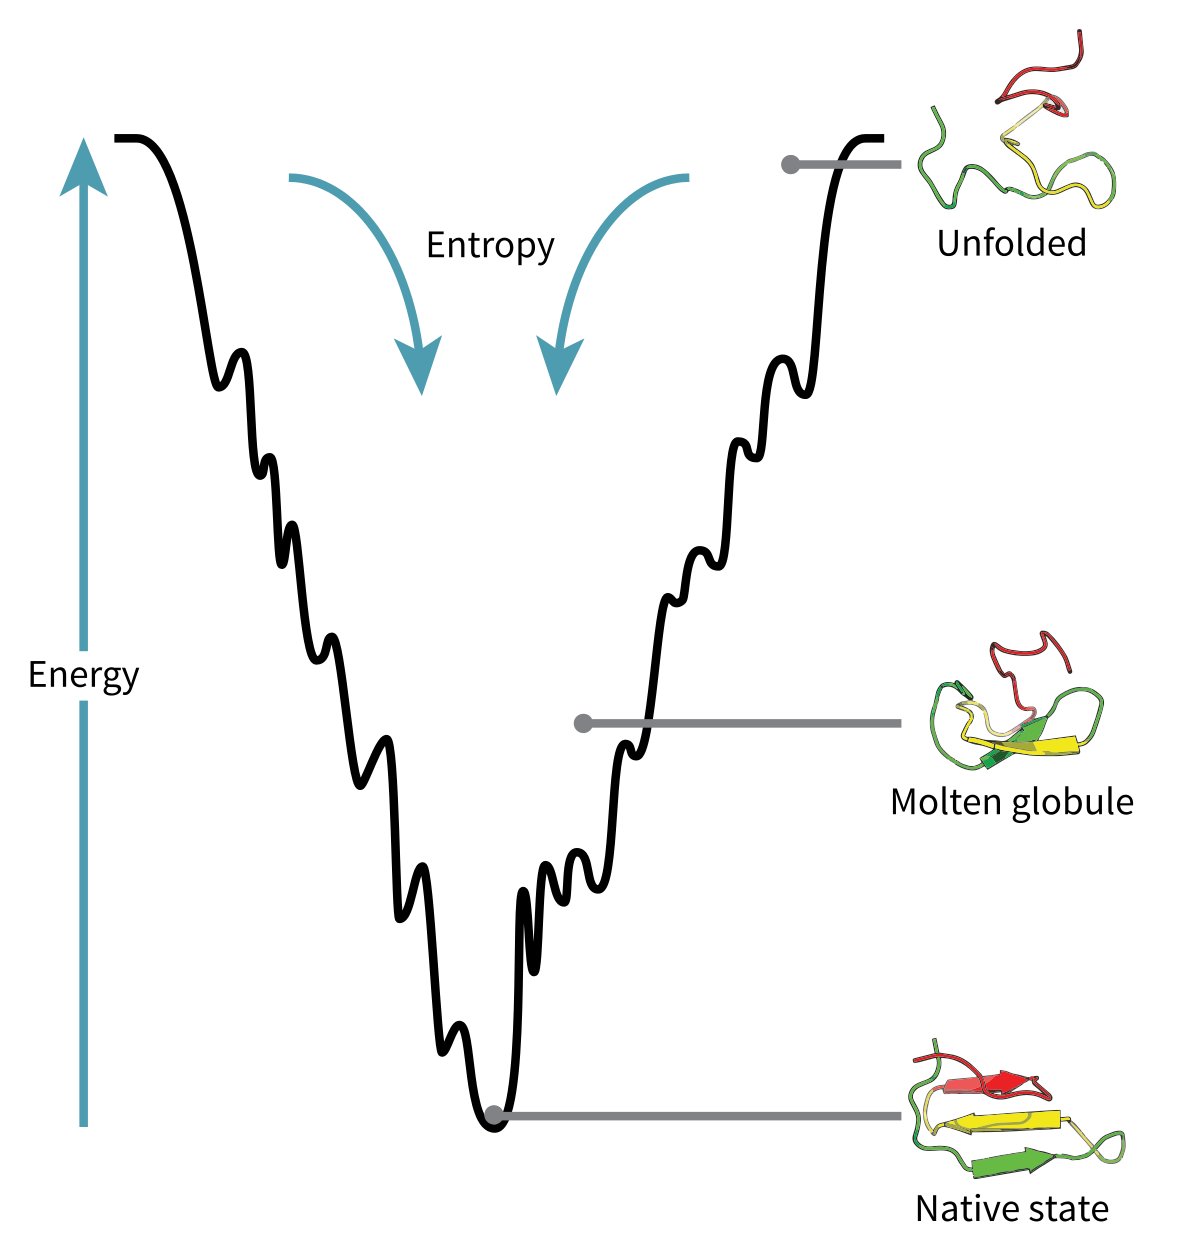
\includegraphics[width=0.5\textwidth]{introduction_foldingfunnel.png}
    \caption{Schematic of the folding funnel hypothesis \cite{Leopold1992-yf}. Diagram produced by \textcite{Wikipedia-FoldingFunnel} contributors.}
    \label{fig:introduction_foldingfunnel}
\end{figure}

In \textit{ab initio} protein structure prediction, the tertiary structure of a protein is predicted using its primary structure alone. This problem is in its nature identical to finding the lowest-energy state along the protein's energy landscape. However, in an attempt to avoid the Levinthal paradox, different knowledge- and physics-based energy functions coupled with a variety of conformational-search sampling algorithms are employed \cite{Lee2017-oc}. 

Physics-based energy functions use physiochemical force fields typically coupled with Molecular Dynamics simulations to sample the folding trajectory of a protein sequence (true physics-based approaches are computationally intractable because quantum mechanics models would need to be used). Force fields describe parameter sets used to calculate energy potentials for a system of atoms in a simulation run, and include potentials such as van der Waals and electrostatic interactions \cite{Lee2017-oc}. In the context of \textit{ab initio} protein structure prediction, pure physics-based approaches are often less favourable, because the computational complexity to find the lowest free-energy state of a large protein structure remains intractable without the use of supercomputers.

Knowledge-based energy functions rely on empirical energy terms derived from statistics and regularities of experimentally determined structures \cite{Lee2017-oc}. These energy terms can be subdivided into two types, the generic or sequence-independent terms and amino-acid or sequence-dependent terms \cite{Skolnick2006-uv}. The former include terms to describe the backbone hydrogen-bonds and local backbone stiffness of a polypeptide chain. The latter describes terms such as pairwise residue contact potential, distance-dependent atomic contact potential, and secondary structure propensities. However, predicting local or global tertiary structure of a protein sequence using empirical energy terms alone is very difficult. Subtle differences in the local and global environment of a primary structure alongside the subtle differences in primary structures leading to common secondary structure features are very difficult to reproduce in a modelling scenario. Thus, knowledge-based energy functions are often coupled with the assembly of fragments extracted from other protein structures to predict the unknown tertiary structure of the target sequence \cite{Lee2017-oc}. 

The most successful \textit{ab initio} structure prediction protocols use knowledge-based and physics-based energy functions combined with fragment-assembly-based conformational searches to find the lowest free-energy state \cite{Rohl2004-dj,Xu2012-jf,De_Oliveira2017-sg}. To achieve this, these protocols generate many thousands of computationally inexpensive models (``decoys'') with conformations specified with heavy backbone and C\textbeta\ atoms. To sample the energy landscape efficiently and avoid entrapment in local free-energy minima, fragments of varying sizes (typically 3-20 residues) are inserted either at a random positions in the polypeptide chain or sequentially added, followed by multiple rounds of Replica-Exchange Monte Carlo minimization \cite{Raman2009-gc,Xu2012-jf,Blaszczyk2013-nx,Kosciolek2014-bt}.
